\documentclass{beamer}

\mode<presentation>
\usetheme[hideothersubsections]{PaloAlto}
\usecolortheme{seagull}
\usefonttheme{serif}
\pgfdeclareimage[height=1cm]{uni}{HWU_logo}
\logo{\pgfuseimage{uni}}

\usepackage{hyperref}
\usepackage{cleveref}
\usepackage{listings}
\usepackage[square,numbers]{natbib}

\setbeamertemplate{caption}[numbered]
\setbeamertemplate{bibliography item}[text]
\setbeamertemplate{bibliography entry title}{}
\setbeamertemplate{bibliography entry location}{}
\setbeamertemplate{bibliography entry note}{}
\renewcommand\bibfont{\scriptsize}

\lstset{basicstyle=\selectfont\ttfamily\color{white},
  showstringspaces=false,
  commentstyle=\color{red},
  keywordstyle=\color{blue},
  backgroundcolor=\color{black}
}

\title{Introduction to \LaTeX}
\author[OTB \& LF]{Oliver T. Brown \& Liam Fitzgerald}
\institute[HWU]{Heriot-Watt University}
\date[2016-01-26]{26th January 2016}

\begin{document}

\begin{frame}
	\titlepage
\end{frame}

\section{Outline}
\begin{frame}
	\frametitle{Outline}
	\tableofcontents
\end{frame}

\section{What is \LaTeX?}

\subsection[LayTECH]{Pronunciation}
\begin{frame}
\frametitle{What is \LaTeX?}
\framesubtitle{Pronunciation}
\uncover<1->{Every single `Intro to \LaTeX' presentation begins this way...} \vspace{\baselineskip}

\uncover<2->{It is pronounced Lay-tech/Lay-teck, \alert{NOT} Lay-tecks.} \vspace{\baselineskip}

\uncover<3->{(Sometimes Lah-tech/Lah-teck)} \vspace{\baselineskip}

\uncover<4->{(Never Lah-tecks)}
\end{frame}

\subsection{Typesetting Language}
\begin{frame}
\frametitle{What is \LaTeX?}
\framesubtitle{Typesetting Language}
\begin{itemize}
\item Builds on the TeX typesetting program developed in a time before graphical interfaces, the 1970s, by Donald E Knuth.
\item It is a \emph{typesetting language}, not a word-processor (more on that shortly).
\item Designed so that the author's job is just to specify the kind of document they want, and produce the content.
\item In principle a nicely presented document can be produced without the author having ever seen it. Useful on a command line computer system!
\end{itemize}
\end{frame}

\subsection{Not Word}
\begin{frame}
\frametitle{What is \LaTeX?}
\framesubtitle{Not Word}
\emph{All right, but basically it's for writing documents, so why is it different from [MY FAVOURITE WORD PROCESSING SOFTWARE]?}
\vspace{\baselineskip}
\begin{itemize}
\item You use commands to define the style of the document.
\item The document is then \emph{compiled}.
\item You don't get to see what it will look like until it has compiled.
\item You don't necessarily get all that much choice about what it looks like.
\end{itemize}
\end{frame}

\section{How does it work?}

\subsection{Obtaining \LaTeX}
\begin{frame}
\frametitle{How does it work?}
\framesubtitle{Obtaining \LaTeX}
\begin{itemize}
\item \alert{Hold on.} There's a pretty good chance if you're using a uni computer, any kind of linux machine, or you've installed a \LaTeX\ IDE that you already have it installed!
\item Having multiple TeX distributions installed can be quite messy, so it's definitely worth checking.
\item If you definitely don't then the easiest way is probably to download the TeX Live package from \url{http://www.tug.org/texlive/} -- be warned, the download can take some time...
\item More information on obtaining TeX and \LaTeX\ can be found at \url{https://latex-project.org/ftp.html}.
\end{itemize}
\end{frame}

\subsection{Compilation}

\lstset{language=bash}

\begin{frame}[fragile]
\frametitle{How does it work?}
\framesubtitle{Compilation}

Back in the good old days you may have had to enter a command sequence like one of the following...

\begin{lstlisting}[caption={Command sequence for this presentation.}, label={lst:1}]
>> pdflatex intro_latex.tex
>> pdflatex intro_latex.tex
>> evince intro_latex.tex
\end{lstlisting}

\begin{lstlisting}[caption={Command sequence for a document containing BibTeX references.}, label={lst:2}]
>> pdflatex OTB_phdthesis_v00.tex
>> bibtex OTB_phdthesis_v00.tex
>> pdflatex OTB_phdthesis_v00.tex
>> pdflatex OTB_phdthesis_v00.tex
>> evince OTB_phdthesis_v00.tex
\end{lstlisting}

\end{frame}

\begin{frame}
\frametitle{How does it work?}
\framesubtitle{Compilation}

In these more enlightened times you'll almost certainly be using an IDE to write and compile your document, so you probably just have to click the `build' button. As an example, \cref{fig:1} below shows a screenshot of TeXMaker, which I used to create this presentation. You can see it has a `Quick Build' button right at the top, as well as a `View PDF' button. 

\begin{figure}[h!]
\centering
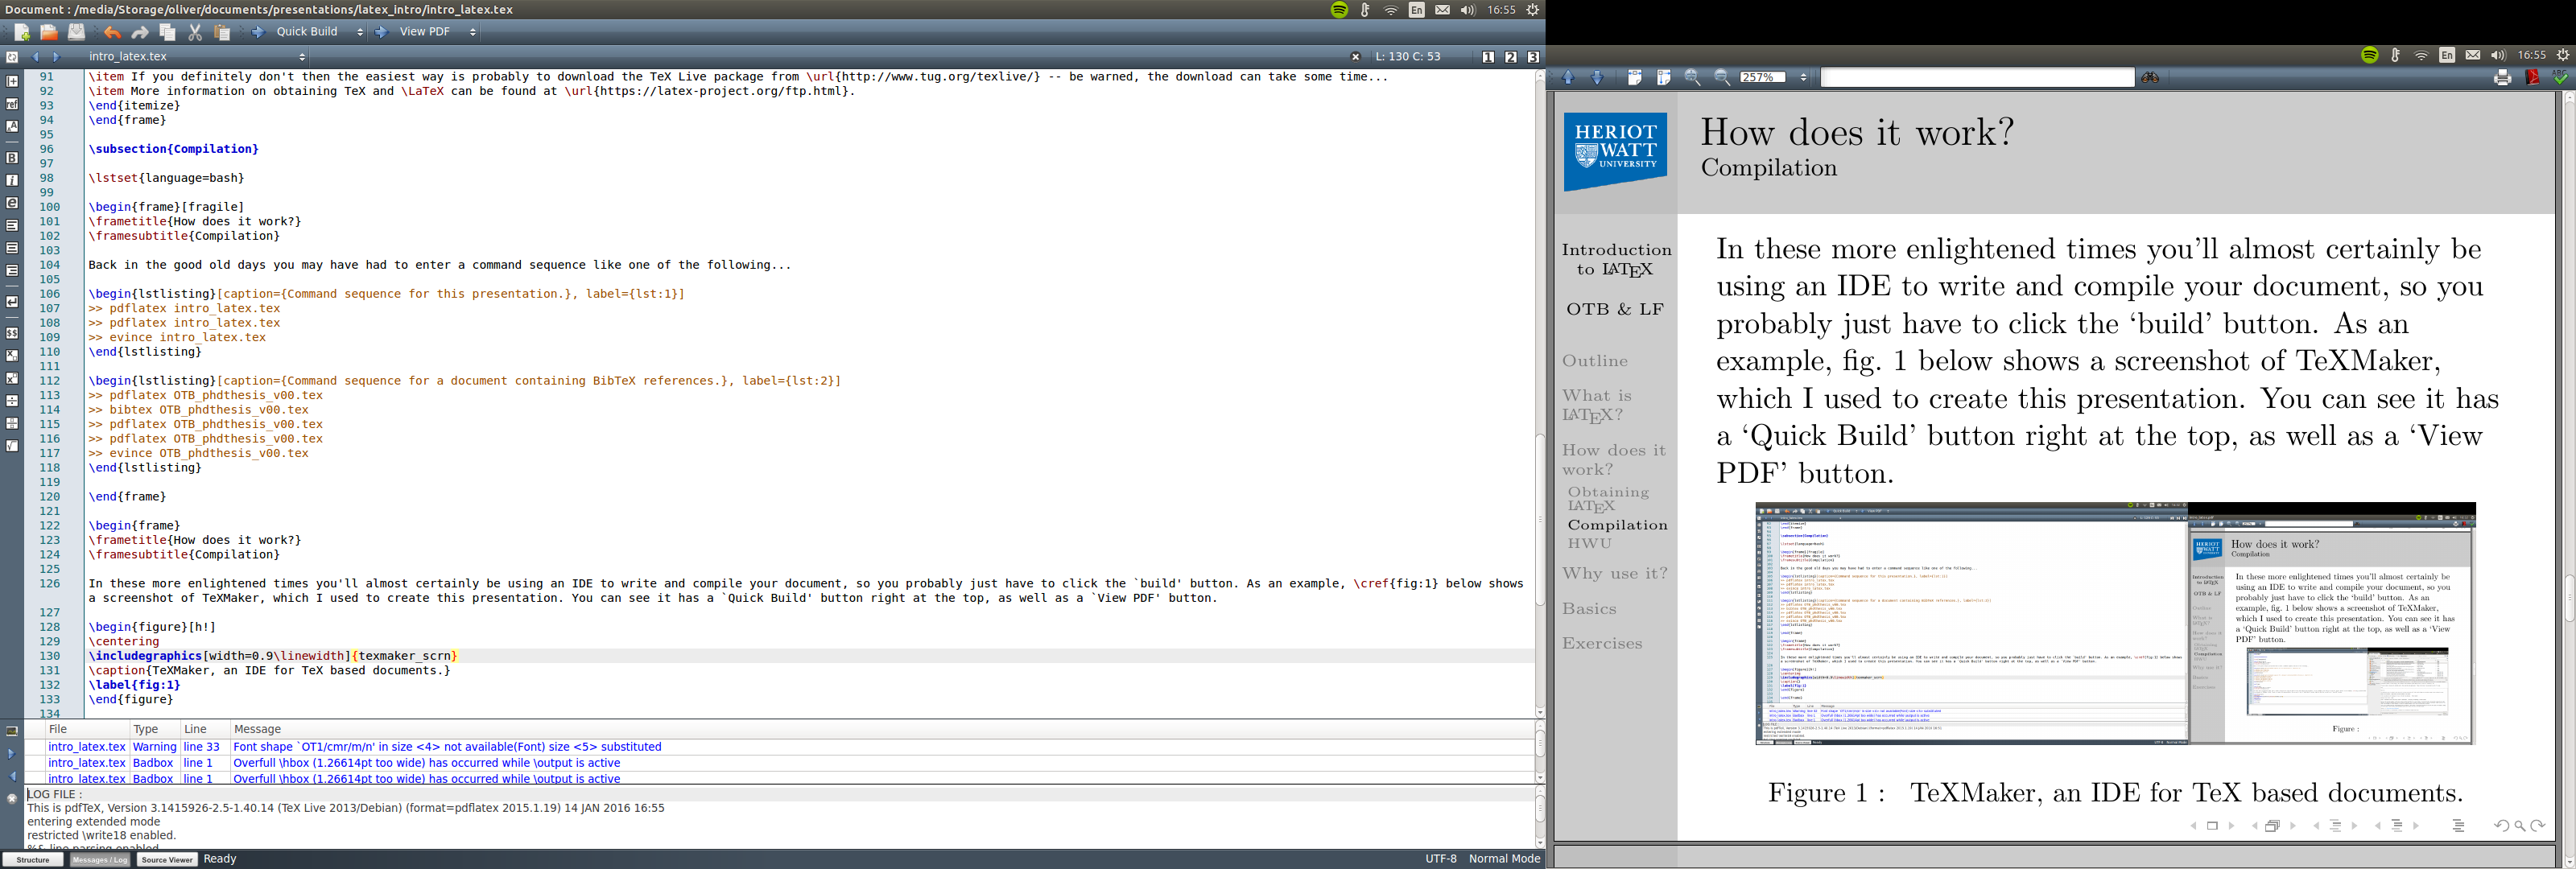
\includegraphics[width=0.9\linewidth]{texmaker_scrn}
\caption{TeXMaker, an IDE for TeX based documents.}
\label{fig:1}
\end{figure}

\end{frame}

\subsection[HWU]{Using \LaTeX\ at Heriot-Watt}
\begin{frame}
\frametitle{How does it work?}
\framesubtitle{Using \LaTeX\ at Heriot-Watt}
The most important thing to know for now of course, is how exactly to use \LaTeX\ on the uni system.

** ASK DAWN IF THIS IS ACTUALLY IMPORTANT **
\end{frame}

\section{Why use it?}

\subsection[Cons]{Disadvantages}
\begin{frame}
\frametitle{Why use it?}
\framesubtitle{Disadvantages}

\begin{itemize}
\item `Programming' is scary!
\item I can't see what I'm doing!
\item Graphics handling is painful.
\item Tables are a faff.
\item The TeX ecosystem is quite diverse with many distributions, IDEs, packages -- which do you choose?
\item For the above reason, portability can be an issue.
\item Intermediate files can cause a lot of clutter (use IDE's `clean' tool).
\item Little to no support for multimedia (that I know of).
\end{itemize}
\end{frame}

\subsection[Pros]{Advantages}
\begin{frame}
\frametitle{Why use it?}
\framesubtitle{Advantages}

\begin{itemize}
\item Typesetting maths: \(\mathcal{L}\{\rho\} = -i[\hat{H}, \rho] - \frac{\gamma}{2}\left(2 \hat{a}\rho\hat{a}^{\dagger} - \hat{a}^{\dagger}\hat{a}\rho - \rho\hat{a}^{\dagger}\hat{a}\right)\)
\item Powerful referencing tool: BibTeX
\item Label system makes cross-referencing easy.
\item Low file-size, so version control systems like Git can be used.
\item Low file-size so large documents won't crash!
\item Many journals provide standard article templates.
\item In principle allows a very high degree of control over document layout.
\end{itemize}
\end{frame}

\section{Basics}
\lstset{
  language={TeX},
  basicstyle=\selectfont\ttfamily\color{black},
  showstringspaces=false,
  commentstyle=\color{blue},
  keywordstyle=\color{green},
  backgroundcolor=\color{white}
}

\begin{frame}[fragile]
\frametitle{Basics}
\framesubtitle{Preamble}
So what about the language itself? The following is a pretty standard `preamble' for scientific documents:
\begin{lstlisting}[label={lst:3}]
\documentclass[a4paper,twoside]{article}

\usepackage[margin=1.75cm]{geometry}
\usepackage{amsmath}
\usepackage{amssymb}
\usepackage{graphicx}
\usepackage{hyperref}
\usepackage{cleveref}
\end{lstlisting}
\end{frame}

\begin{frame}[fragile]
\frametitle{Basics}
\framesubtitle{\textbackslash begin\{document\}}
\begin{lstlisting}[label={lst:4}]
\author{Oliver Thomson Brown}
\title{Matrix Product States}
\date{2016-01-15}

\begin{document}

\maketitle

\tableofcontents

	...
	
\end{document}
\end{lstlisting}
\end{frame}

\begin{frame}[fragile]
\frametitle{Basics}
\framesubtitle{Commands}
\begin{itemize}
\item \verb:\: identifies a command sequence (\verb:\textbackslash: typesets a \textbackslash).
\item \verb:\: is also an escape sequence for typesetting symbols like \{, \}, and \&.
\item \verb:\\: \emph{requests} a newline.
\item \verb:\emph{}: for \emph{italics}, \verb:\textbf{}: for \textbf{bold}.
\item \verb:\section{Section Title}: creates sections which are automatically labelled and included in your table of contents.
\item \verb:\label{}: can be used to label sections, figures, equations, etc. and is \emph{highly} recommended. Especially in conjunction with the cleveref and hyperref packages.
\end{itemize}
\end{frame}

\begin{frame}[fragile]
\frametitle{Basics}
\framesubtitle{Mathematics}
Inline maths:
\begin{verbatim}
    \( E = \frac{1}{2} mv^{2} \)
\end{verbatim}
One of Einstein's discoveries was the equation \(E = \frac{1}{2}mv^{2}\), equating energy and mass. \\
\vspace{\baselineskip}
Display maths:
\begin{verbatim}
\begin{equation}
    \rho = | \psi \rangle \langle \psi |
\label{eq:1}
\end{equation}
\end{verbatim}
\begin{equation}
\rho = | \psi \rangle \langle \psi |
\label{eq:1}
\end{equation}
\end{frame}

\begin{frame}[fragile]
\frametitle{Basics}
\framesubtitle{Images}
Honestly, probably the weakest part of working with \LaTeX...

\begin{lstlisting}[label={lst:4}]
\begin{figure}[h!]
	\centering
	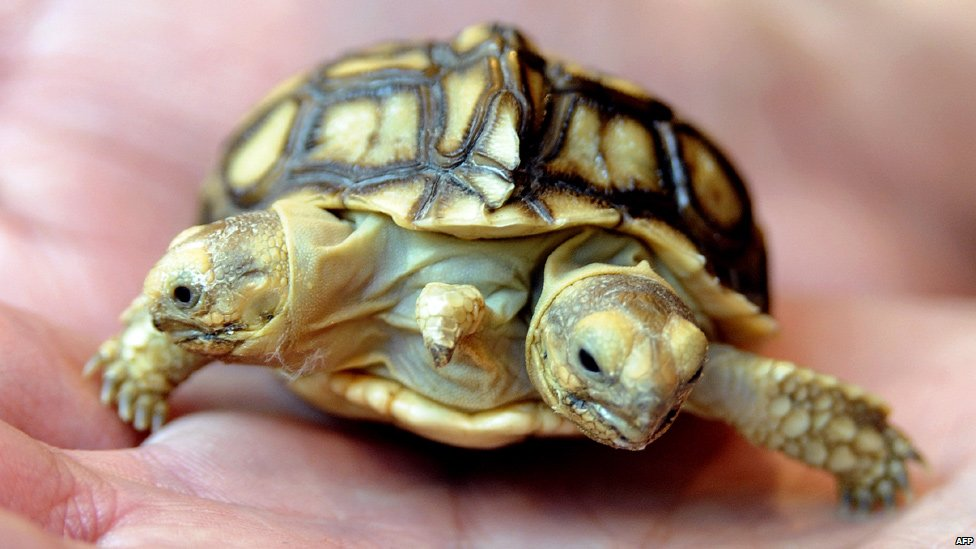
\includegraphics[width=0.6\linewidth]
	{two_head_tortoise}
	\caption{A two-headed tortoise!}
	\label{fig:2}
\end{figure}
\end{lstlisting}

\begin{figure}[h!]
	\centering
	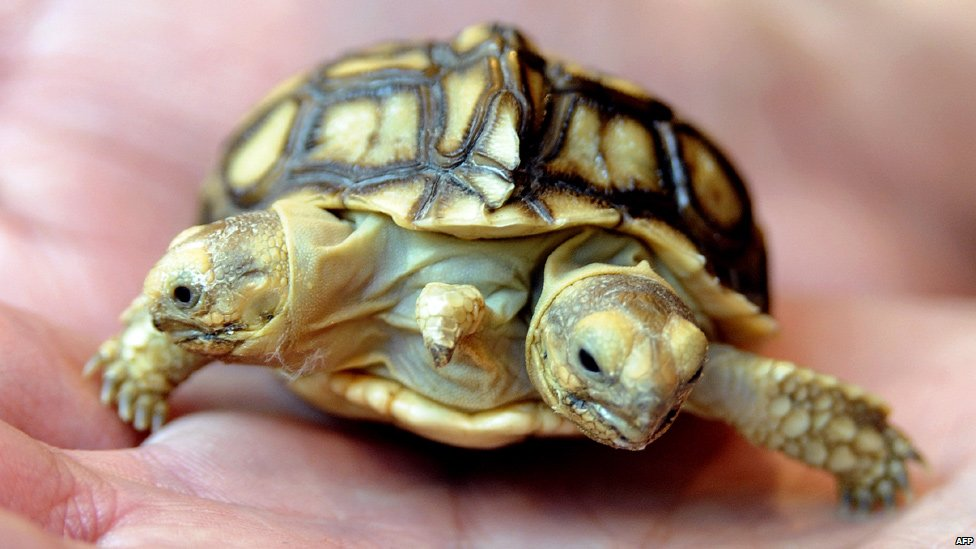
\includegraphics[width=0.5\linewidth]{two_head_tortoise}
	\caption{A two-headed tortoise!}
	\label{fig:2}
\end{figure}
\end{frame}

\begin{frame}[fragile]
\frametitle{Basics}
\framesubtitle{BibTeX}

BibTeX is a simple to use, but powerful referencing tool. First you need a .bib file in the same folder -- part of intro\_latex.bib is shown here:

\begin{lstlisting}[label={lst:5}]
@book{NR,
year={2007},
author={Press, William H. and Teukolsky, Saul A. and Vetterling, William T. and Flannery, Brian P.},
title={Numerical Recipes -- The Art of Scientific Computing},
publisher={Cambridge University Press},
edition={3E},
}
\end{lstlisting}

The format is quite straightforward, and many journals provide BibTeX citations which you can copy and paste into your own .bib file. In this example `NR' is the citation label.

\end{frame}

\begin{frame}[fragile]
\frametitle{Basics}
\framesubtitle{BibTeX}
Then you need to include a \verb:\bibliographystyle{}: command, and \verb:\bibliography{}: in the document:
\begin{lstlisting}[label={lst:6}]
\bibliographystyle{acm}
\bibliography{intro_latex}
\end{lstlisting}

You then simply use the \verb:\cite{citation-label}: command to reference things like this conference paper I wrote \cite{Bea13}, or the book \emph{Numerical Recipes} \cite{NR}.
\end{frame}

\begin{frame}
\frametitle{Basics}
\framesubtitle{References}
\LaTeX\ and BibTeX take care of the rest for you...

\bibliographystyle{acm}
\bibliography{intro_latex}

Unsurprisingly, many journals also provide their own BibTeX style files. Always worth checking before you try and format references manually!
\end{frame}

\section{Resources}
\begin{frame}
\frametitle{Resources}
\begin{itemize}
\item Source for this presentation, as well as examples and exercises can be downloaded from: \url{https://github.com/otbrown/HWU16_latex}.
\item Main \LaTeX\ project website: \url{http://latex-project.org/}.
\item The \LaTeX\ wikibook is great for quickly looking up standard commands -- especially Mathematics: \url{https://en.wikibooks.org/wiki/LaTeX}
\item For BibTeX, the main Wikipedia page is a little more useful: \url{https://en.wikipedia.org/wiki/BibTeX}.
\item Ask! There are plenty of \LaTeX\ users in the department (especially theorists!) so if you can't work out how to do something ask around.
\end{itemize}

\alert{Google is your friend.}
\end{frame}

\section{Exercise}
\begin{frame}
\frametitle{Exercise}
\framesubtitle{Template Document}

\begin{itemize}
\item Create a template \LaTeX\ `article' document which you can copy-paste from/refer to in the future.
\item Include anything you think you might want to do again in the future -- equations, tables, images... If you get stuck check the Resources on the previous slide, or ask one of us!
\item Play around with packages a bit too. In particular see what happens if you don't use the \emph{geometry} package to control the margin size.
\item You can find an example document in the `example' folder, in the GitHub repo (\url{https://github.com/otbrown/HWU16_latex}).
\end{itemize}

\end{frame}

\end{document}